%----------------------------------------------------------------------------------------
%    PACKAGES AND THEMES
%----------------------------------------------------------------------------------------

\documentclass[aspectratio=169,xcolor=dvipsnames]{beamer}
\usetheme{SimplePlus}

\usepackage{hyperref}
\usepackage{graphicx} % Allows including images
\usepackage{booktabs} % Allows the use of \toprule, \midrule and \bottomrule in tables

%----------------------------------------------------------------------------------------
%    TITLE PAGE
%----------------------------------------------------------------------------------------

\title{Cubical Complexes}
\subtitle{}

\author{Enei Sluga, Simon Hehnen}

\institute
{
    Faculty of Computer and Information Science \\
    University of Ljubljana % Your institution for the title page
}
\date{\today} % Date, can be changed to a custom date

%----------------------------------------------------------------------------------------
%    PRESENTATION SLIDES
%----------------------------------------------------------------------------------------

\begin{document}

\begin{frame}
    % Print the title page as the first slide
    \titlepage
\end{frame}

\begin{frame}{Overview}
    \tableofcontents
\end{frame}

%------------------------------------------------
\section{Intdroduction}
%------------------------------------------------

\begin{frame}{Introduction}
    \textbf{What are Cubical Complexes?}
    \begin{itemize}
        \item Cubical complexes are structures built using cubes as building blocks.
        \item They generalize simplicial complexes by using:
        \begin{itemize}
            \item \textbf{0-cubes:} Vertices
            \item \textbf{1-cubes:} Edges (horizontal or vertical)
            \item \textbf{2-cubes:} Squares
        \end{itemize}
        \item Applications in image analysis and higher-dimensional data.
    \end{itemize}
\end{frame}

%------------------------------------------------

\begin{frame}{Generation of Cubical Complexes}
    \textbf{Steps to Construct Cubical Complexes:}
    \begin{enumerate}
        \item Define a grid structure (e.g., \( n \times n \)).
        \item Assign coordinates to vertices, edges, and squares.
        \item Ensure orientation is consistent (e.g., positive rotational order for squares).
        \item Apply boundary conditions for chain construction.
    \end{enumerate}

    \vspace{1em}
    \textbf{Key Feature:} Each cube is labeled systematically for easy computation.
\end{frame}

%------------------------------------------------

\begin{frame}{Example: 2D-Torus}
    \textbf{Generating a 2D-Torus using Cubical Complexes}
    \begin{itemize}
        \item Represent a torus as a 2D grid with periodic boundary conditions.
        \item Connect edges of the grid (left to right, top to bottom).
        \item Visualize the transformation from a grid to a torus shape.
    \end{itemize}

    \vspace{1em}
    \centering
    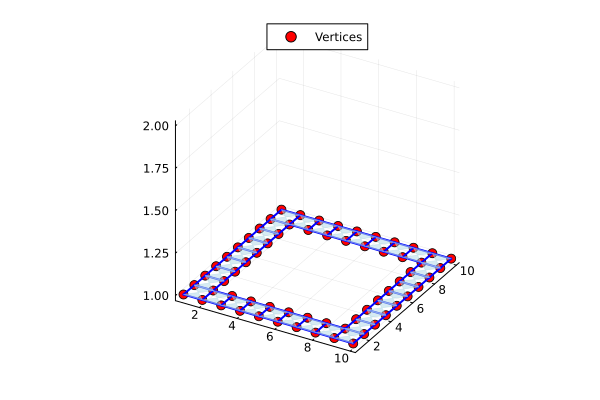
\includegraphics[width=0.5\textwidth]{torus2D.png} % Replace with actual image path
\end{frame}

%------------------------------------------------

\begin{frame}{Example: 3D-Torus}
    \textbf{Generating a 3D-Torus (filled) using Cubical Complexes}
    \begin{itemize}
        \item Represent a torus as a 2D grid with periodic boundary conditions.
        \item Connect edges of the grid (left to right, top to bottom).
        \item Visualize the transformation from a grid to a torus shape.
    \end{itemize}

    \vspace{1em}
    \centering
    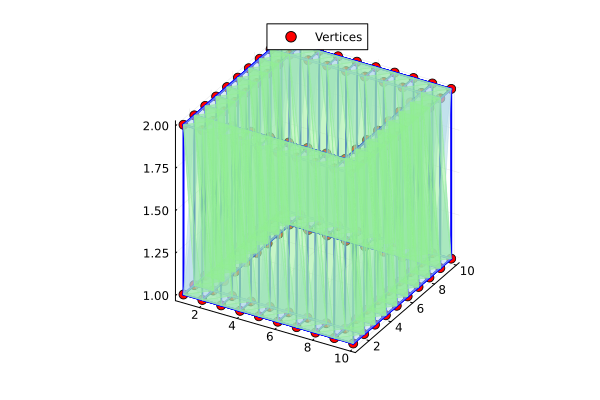
\includegraphics[width=0.5\textwidth]{torus3D.png} % Replace with actual image path
\end{frame}

%------------------------------------------------
\section{Homology}
%------------------------------------------------

\begin{frame}{Homology}
    TODO explain Homology (You)
\end{frame}

%------------------------------------------------
\section{Examples}
%------------------------------------------------

\begin{frame}{Images}
    TODO show some examples (e.g. images, complex objects etc.) (Together)
\end{frame}

\begin{frame}{References}
    \footnotesize
    \bibliography{reference.bib}
    \bibliographystyle{apalike}
\end{frame}
\end{document}